\section{Introduction}

% UMTS Network

% RRC State Machine
3G cellular data networks have recently witnessed rapid growth, especially due to the emergence of smartphones. In this paper, we focus on the UMTS (the Universal Mobile Telecommunications System) 3G network, which is among the most popular 3G mobile communication technologies. However, the bottleneck of the internet resides in the first hop of the network, and large amount of lower layer retransmission could cause significant latency~\cite{bufferbloat}. 3G network has a bad reputation for slow initial network connection~\cite{3g.slow}.

3G network systems operate under more radio resource constraints. To efficiently utilize the limited radio resources, UMTS introduces for each user equipment (UE, for instance, a smartphone) a radio resource control (RRC) state machine, such as in Figure~\ref{fig:rrc.state.machine}, that determines radio resource usage affecting device energy consumption and user experience~\cite{spec-3G-RRC}. Usually a UE (user equipment) can be in one of three states, each with different amount of allocated radio resources. The transitions between states also have significant impact on the UMTS system. 

\begin{figure}[h!]
\centering
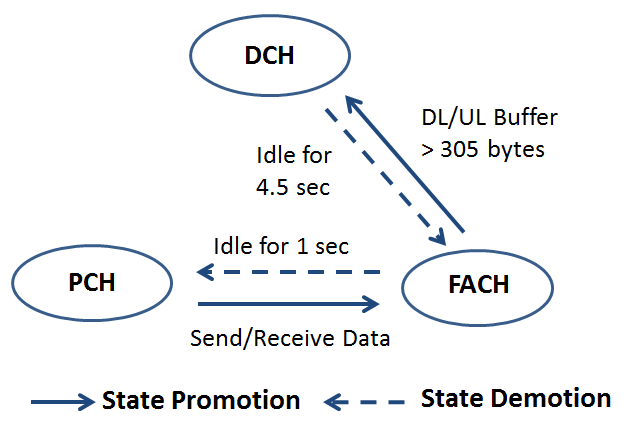
\includegraphics[width=0.45\textwidth]{figs/rrc_state.png}
\caption{RRC State Machine for the 3G UMTS network for T-Mobile}
\label{fig:rrc.state.machine}
\end{figure}

The network topology provides a nature isolation between different layers. The design of transport layer protocol doesn't require the knowledge of lower layer information. However, the abstraction of the design could lead to sub-optimal scenario, i.e. large significant latency will occur during the RRC state transition. Since the root cause of the abnormal delay behavior resides in the data link layer (i.e. RLC, radio link control, layer), the visibility of lower layer information will help us identify the root cause of the bizarre behavior in upper layer. Fortunately, we have a real-time monitoring tool, called QxDM as in Figure~\ref{fig:qxdm}, to enable use capture the radio traffic information cross multiple layers. Therefore, cross layer analysis over QxDM logs would help us have a in-depth understanding the correlation between different layers, and identify the root cause of abnormal latency behaviors during the initial state of data transmission.

\begin{figure}[h!]
\centering
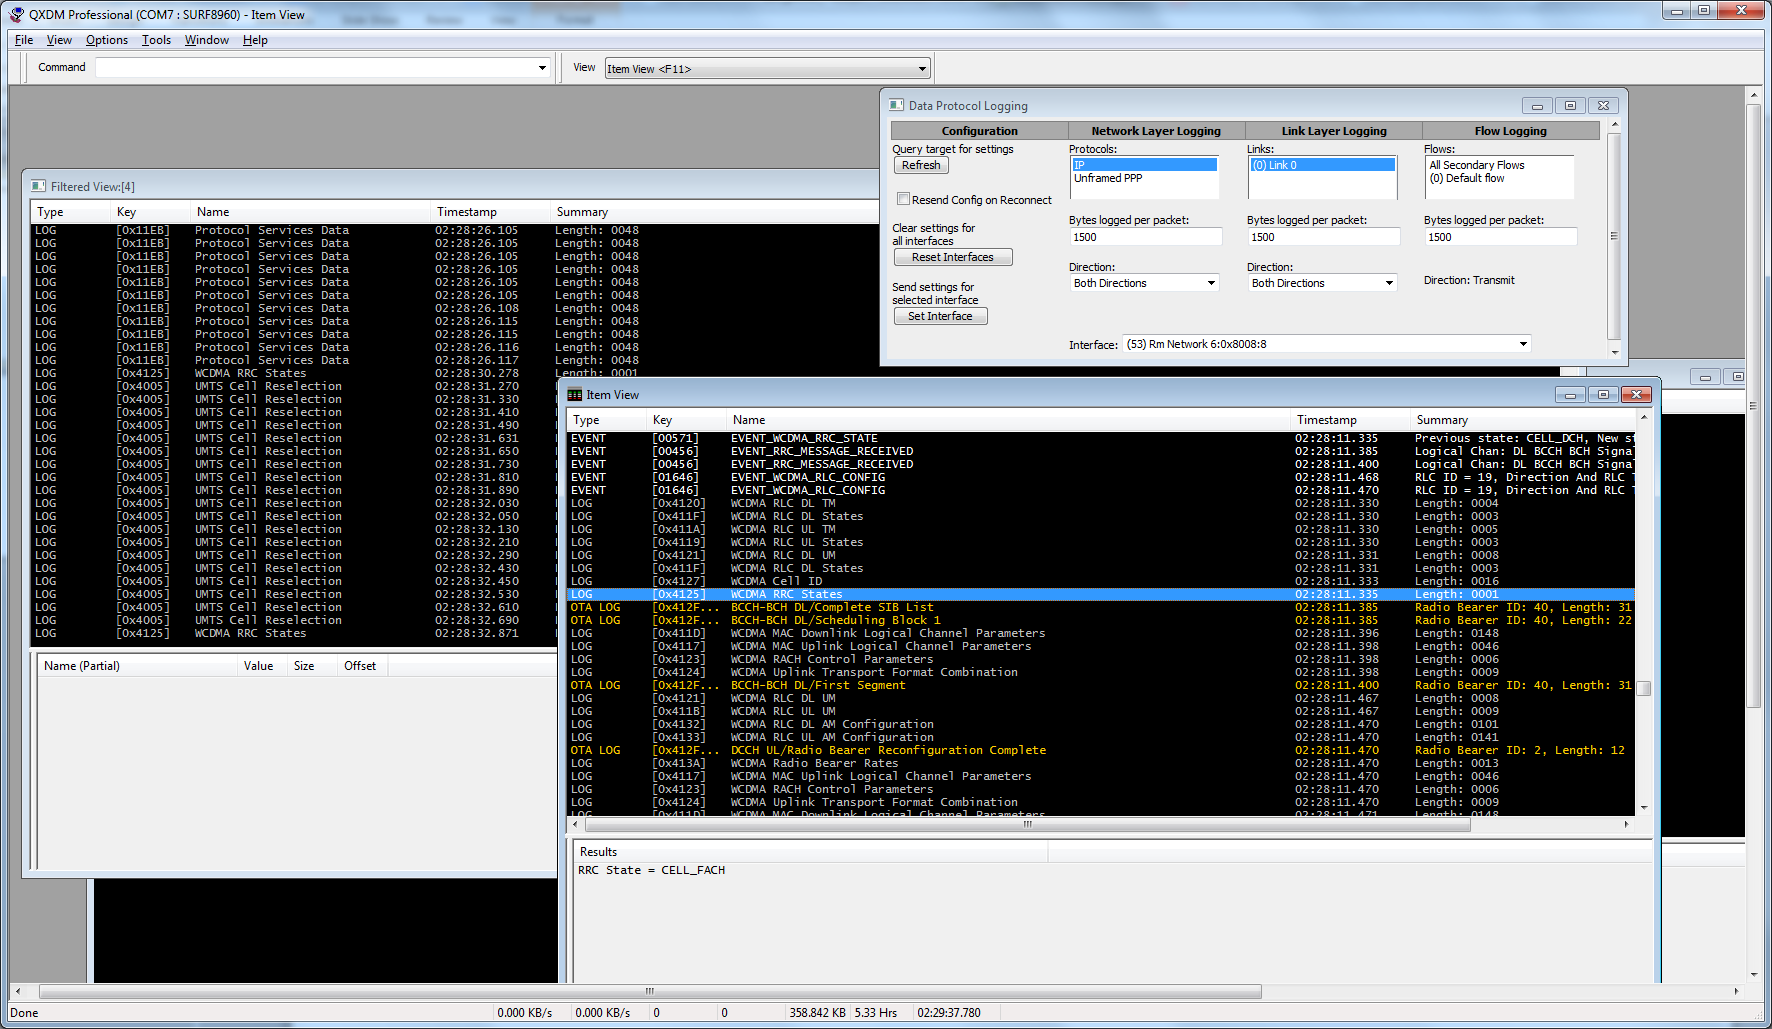
\includegraphics[width=0.45\textwidth]{figs/QxDM.png}
\caption{Ongoing monitoring and logging activities on QxDM}
\label{fig:qxdm}
\end{figure}

\label{sec:intro}

We propose an improvement to how RLC currently behaves based on our findings. To avoid extra retransmissions that occur during the poorly-performing FACH state and FACH-state transitions observed, the application could batch the data transmission to reduce the possible number of transmissions in these states.  To address this RLC retransmission delay issue, we propose a RLC \emph{Fast Re-Tx} mechanism that actively responds to the RLC PDU loss signals. By simulating this fast retransmission mechanism using real QXDM traces, we apply a cost-benefit analysis and find that \emph{Fast Re-Tx} could reduce RLC latency by up to 35.69\% when these poorly-performing FACH states occur. 
